\documentclass[varwidth=true, border=2pt]{standalone}
\usepackage{tkz-euclide}
\usepackage{tikz}
\usetikzlibrary{decorations.pathreplacing}


\begin{document}
\usetkzobj{all}
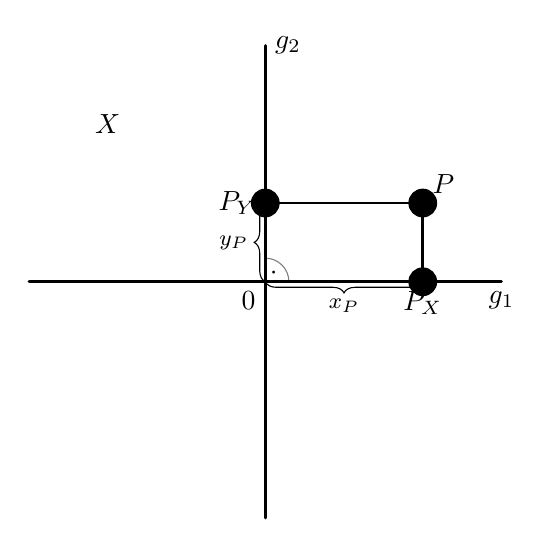
\begin{tikzpicture}
    \tkzSetUpPoint[shape=circle,size=10,color=black,fill=black]
    \tkzSetUpLine[line width=1]
    \tkzDefPoints{0/0/O, 1/0/X, 0/1/Y, 2/1/P}

    \tkzMarkAngle[fill=green!20,size=0.3cm,opacity=.5](X,O,Y)
    \tkzLabelAngle[pos=0.15](X,O,Y){$\cdot$}

    \tkzDrawLine[add=3 and 2](O,X)
    \tkzLabelLine[below,pos=3](O,X){$g_1$}
    \tkzLabelLine[right,pos=3](O,Y){$g_2$}
    \tkzDrawLine[add=3 and 2](O,Y)

    \tkzDefLine[orthogonal=through P,/tikz/overlay](O,X) \tkzGetPoint{helper}
    \tkzInterLL(O,X)(P,helper) \tkzGetPoint{xp}
    \draw [decorate,decoration={brace,amplitude=4pt,mirror}]
        (O) -- (xp) node [black,midway,xshift=0cm, yshift=-0.3cm] 
        {\footnotesize $x_P$};

    \tkzDefLine[orthogonal=through P,/tikz/overlay](O,Y) \tkzGetPoint{helper}
    \tkzInterLL(O,Y)(P,helper) \tkzGetPoint{yp}
    \draw [decorate,decoration={brace,amplitude=4pt}]
        (O) -- (yp) node [black,midway,xshift=-0.4cm] 
        {\footnotesize $y_P$};

    \tkzDrawPolygon(O,xp,P,yp)

    \tkzLabelPoint[above right](P){$P$}
    \tkzLabelPoint[below left](O){$0$}
    \tkzLabelPoint[below](xp){$P_X$}
    \tkzLabelPoint[left](Y){$P_Y$}
    \node at ($(-2,2)$){$X$};
    \tkzDrawPoints(P,Y,xp)
\end{tikzpicture}
\end{document}
